\chapter{Aufgabenanalyse}\label{ch:aufgabenanalyse}


\section{Interpretation der Aufgabe}\label{sec:interpretation-der-aufgabe}
Zur Auswertung von Signalen eines optischen Autokorrelators soll ein Programm entwickelt werden.
Der Autokorrelator liefert fortlaufend Daten, die vom Programm eingelesen, verarbeitet und ausgegeben werden.
Weil diese Schritte für unterschiedliche Datensätze unterschiedliche Laufzeiten haben, sollen sie in voneinander unabhängigen Threads laufen.

Die einzelnen Datensätze werden zum Test in zehn unterschiedlichen Textdateien zur Verfügung gestellt.
Diese sind durchnummeriert von null bis neun und haben die folgende Namenskonvention:
\begin{center}
    <nummer>.txt
\end{center}
Ein Datensatz enthält jeweils $N$ Messdaten, die aus zwei positiven Ganzzahlen bestehen.
Die erste Zahl steht dabei für die Intensität des Messsignals und wird im Folgenden als y-Wert interpretiert.
Die zweite Zahl bezeichnet die Spielposition und wird als \~x-Wert interpretiert.
Der Spiegel ist eine Komponente des Autokorrelators die vor und zurück bewegt werden kann, um das Output-Signal zu manipulieren.

Der einlesende Thread soll die zehn Textdateien in chronologischer Reihenfolge einlesen und in eine geeignete Datenstruktur überführen.
Wenn zehnte Datei fertig bearbeitet wurde, soll wieder bei ersten begonnen werden.
Dieses Verhalten wird fortgesetzt bis ein Signal zum Programmabbruch empfangen wird.
Es soll hier das Verhalten im produktiven Betrieb simuliert werden, in dem nicht nur zehen Datensätze bearbeitet werden, sondern fortlaufend neue Datensätze vom Autokorrelator produziert werden.
Der Einlese-Thread stellt jeden Datensatz für 0,05 Sekunden zur Abholung über eine Schnittstelle zur Verfügung.

Der Verarbeitungs-Thread holt sich über diese Schnittstelle Datensätze, führt diverse Transformationen und Berechnungen durch und sendet die Ergebnisse an den Ausgabe-Thread.
Es werden nur Datensätze verarbeitet, die die Verarbeitung vorher noch nicht durchlaufen haben.
Auch die Verarbeitung läuft bis ein Signal zum Programmabbruch empfangen wird.

Gleiches gilt für den Ausgabe-Thread.
Dieser bietet eine Schnittstelle, über die verarbeitete Datensätze angenommen werden.
Die Ergebnisse werden wieder in eine Textdatei geschrieben.
Wenn die Ausgabe eines Datensatzes erfolgreich war, wird das an zentraler Stelle vermerkt.
So kann erkannt werden, wenn alle Eingabedateien erfolgreich verarbeitet und ausgegeben wurden.
Dann ist das Kriterium zum Programmende erreicht und alle Threads können beendet werden.

\section{Mathematische Beschreibung der vier Algorithmen}\label{sec:mat-beschreibung}
Die Verarbeitung wird jeweils auf einem einzelnen Datensatz aus der Eingabe durchgeführt.
Dieser Datensatz kann beschrieben werden durch eine Liste aus $N$ Datenpunkten, die jeweils einen \~x- und einen y-Wert beinhalten.
Aus den Datenpunkten wird in vier Verarbeitungsschritten das gewünschte Ergebnis gewonnen.

\subsection{Umrechnung und Normierung der Daten}\label{subsec:umrechnung-und-normierung}
Im ersten Schritt werden sowohl die \~x-Werte, als auch die y-Werte manipuliert.

Die y-Werte werden normiert, indem jeder einzelne y-Wert durch den maximalen y-Wert geteilt wird.
Also setzte $y_{max} = max(\bm{y})$ und berechne
\[
    y_k = \frac{y_k}{y_{max}}, \forall k \in [0, N - 1]
\]
Dafür werden zwei einfache Iterationen über die Datenliste benötigt:
Die erste zum Bestimmen des maximalen y-Wertes und die zweite um jeden y-Wert mit dem Maximum zu skalieren.

Jeder \~x-Wert wird durch die folgende Transformation in die Einheit Pikosekunden [ps] umgerechnet:
\[
    \tilde{x}_k = \frac{\tilde{x}_k}{2^{18} - 1} \cdot 266.3 - 132.3, \forall k \in [0, N - 1]
\]
Dieser Schritt benötigt lediglich eine Iteration und kann parallel zur zweiten Iteration der y-Normierung durchgeführt werden.

\subsection{Glättung der Daten}\label{subsec:glaettung}
Aufgrund von Messungenauigkeiten liegen die Sensordaten nicht in stetiger Form vor (siehe Abbildung~\ref{fig:glaettung}).
Deshalb wird nun jeder der \~x-Werte durch einen gleitenden Mittelwert aus seiner Umgebung ersetzt.
Für den gleitenden Mittelwert wird jedes Mal ein arithmetisches Mittel aus \~x-Werten in einem Intervall bestimmt.
Die Details dieser Berechnung werden nun genauer erläutert.

Im ersten Schritt wird die Breite des Intervalls festgelegt.
Diese hängt von der Anzahl der Datenpunkte $N$ ab.
\[
    n =
    \begin{cases}
        \lfloor0.002 \cdot N \rfloor - 1 & , \text{wenn} \lfloor0.002 \cdot N \rfloor \text{gerade} \\
        \lfloor0.002 \cdot N \rfloor     & , \text{wenn} \lfloor0.002 \cdot N \rfloor \text{ungerade}
    \end{cases}
\]
Diese Breite wird nun halbiert, und gibt die distanz in jeweils eine x-Richtung an.
\[
    \tau = \frac{n - 1}{2}
\]
Nun wird mit folgender Formel der gleitende Mittelwert für alle $N$ Datenpunkte berechnet.
\[
    x_k = \frac{1}{n} \sum_{i = 0}^{n - 1} \tilde{x}_{k-\tau+i}
\]
Für einen Punkt $k$ werden jeweils die $\tau$ vorherigen \~x-Werte, die $\tau$ nachfolgenden \~x-Werte und der aktuelle Wert an der Stelle $k$ aufaddiert.
Diese Summe wird dann durch die Anzahl der Summanden geteilt.
Wenn das für alle $N$ gemacht wurde, kann im Graph eine Glättung erkannt werden (siehe Abbildung~\ref{fig:glaettung}).

Bei der Berechnung des gleitenden Mittelwertes muss an den Rändern der Datenliste besonders Acht gegeben werden.
Gilt für den Index $k-\tau+i < 0$ oder $k-\tau+i > N + 1$, dann kann hier kein \~x-Wert zugeordnet werden.
Ein solcher Fall tritt z.B. auf, wenn $x_0$ berechnet werden soll.
Dann ist es sinnvoll den Mittelwert aus allen Punkten im Intervall zu bilden, bei denen ein \~x-Wert zugeordnet werden kann.
Da dadurch die Anzahl der Summanden geringer sein kann, muss der skalierende Faktor $\frac{1}{n}$ natürlich angepasst werden.


\begin{figure}[htb]
    \centering
    \begin{minipage}{.5\textwidth}
        \centering
        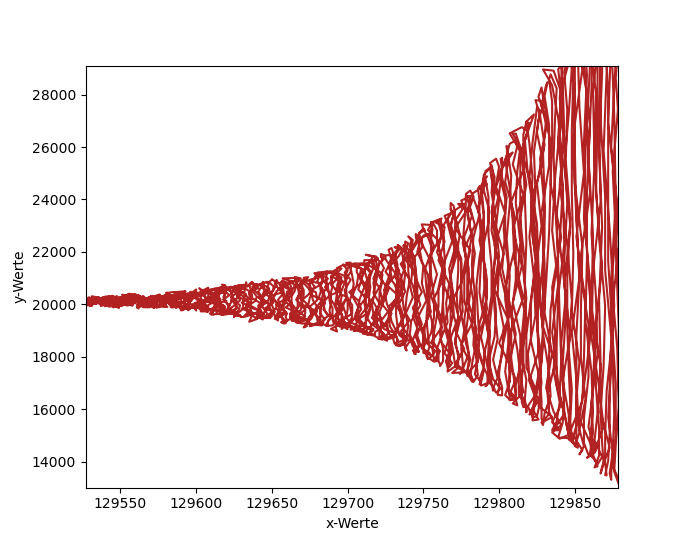
\includegraphics[width=\linewidth]{images/EingabeNichtGlatt}
    \end{minipage}%
    \begin{minipage}{.5\textwidth}
        \centering
        \includegraphics[width=\linewidth]{images/Geglättet}
    \end{minipage}
    \caption{Ausschnitt des eines Datensatzes vor (links) und nach (rechts) Skalierung, Normierung und Glättung.}
    \label{fig:glaettung}
\end{figure}


\subsection{Obere Einhüllende}\label{subsec:ober-einh}
Es soll nun eine Funktion bestimmt werden, die die gegebenen Daten nach oben hin abschätzt.
Diese wird für spätere Berechnungen benötigt.
Die Funktion wird als Feld der länge $N$ gespeichert.
Eine solche Funktion kann durch Bestimmen von lokalen Maxima bestimmt werden, was aber recht aufwändig ist.
Unter der Annahme, dass die Eingabedaten immer die Glockenform wie in Abbildung~\ref{fig:eingabe-plot} haben, kann die obere Einhüllende durch eine einfachere Methode approximiert werden.
\begin{figure}[htb]
    \centering
    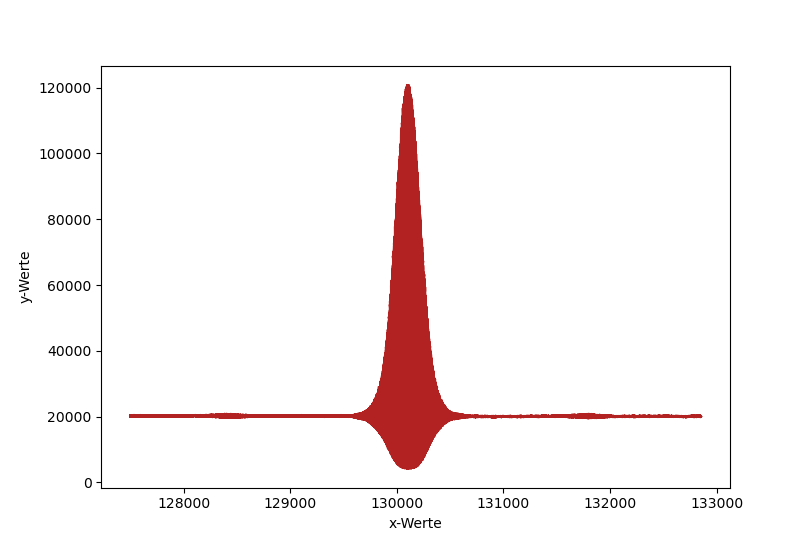
\includegraphics[width=0.8\linewidth]{images/EingabeInsgesamt}
    \caption{
        Ein Plot eines Datensatzes aus der Eingabe.
    }
    \label{fig:eingabe-plot}
\end{figure}

Im ersten Schritt werden wieder der maximale y-Wert (durch die Normierung sollte dieser nun 1 sein) und sein zugehöriger Index berechnet.

Dann wird vom Anfang der Liste der Datenpunkte (also grafisch von links aus) bis zum Index des Maximums iteriert.
In jedem Iterations-Schritt wird ein Wert der oberen Einhüllenden geschrieben.
Bei diesem Wert handelt es sich wieder um ein y-Maximum, das dynamisch während der Iteration gebildet wird.
Initial hat dieses lokale Maximum den Wert $y_0$.
Jedes Mal, wenn ein höherer y-Wert gefunden wird, überschreibt dieser das lokale Maximum.
Wenn der Index des Maximums erreicht wurde, kann die gleiche Methode vom anderen Ende der Liste wiederholt werden.
Dort wird also das lokale Maximum initial auf $y_{N-1}$ gesetzt.

Zuletzt darf nicht vergessen werden den Wert $y_{max}$ an der zugehörigen stelle in der oberen Einhüllenden einzutragen.

\begin{figure}[htb]
    \centering
    \begin{minipage}{.5\textwidth}
        \centering
        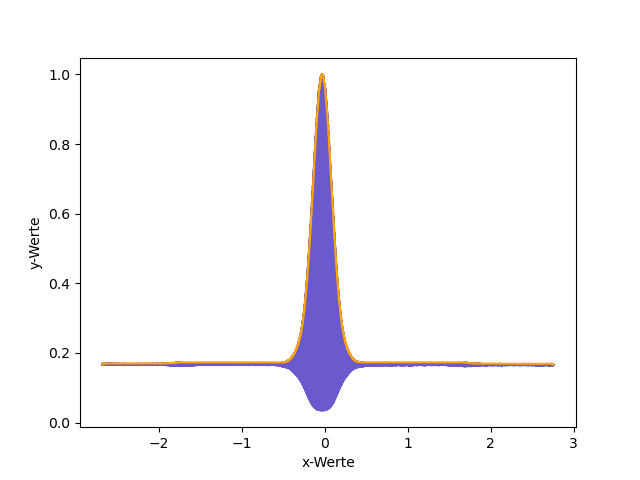
\includegraphics[width=\linewidth]{images/ObereEinhuellende}
    \end{minipage}%
    \begin{minipage}{.5\textwidth}
        \centering
        \includegraphics[width=\linewidth]{images/EinhüllendeNah}
    \end{minipage}
    \caption{Die obere Einhüllende, erstellt durch das beschriebene Verfahren.}
    \label{fig:oberer-einh}
\end{figure}

\subsection{Pulsbreite}\label{subsec:pulsbreite}
Im letzten Schritt der Verarbeitung soll die Pulsbreite berechnet werden.

Zuerst muss dazu die Grundlinie berechnet werden.
Diese berechnet sich als arithmetisches Mittel der y-Werte aus den ersten 1\% der Messpunkte in der Liste.
Also setze
\[
    n = \lfloor0.01 \cdot N \rfloor
\]
und
\[
    Grundlinie = \frac{1}{n} \sum_{k = 0}^{n - 1} y_k
\]
Im Anschluss wird wieder der maximale y-Wert benötigt, um den Punkt auf halber Höhe von Grundlinie zum Maximum zu ermitteln.
\[
    Zielwert = \frac{y_{max} - Grundlinie}{2} + Grundlinie
\]
Nun wird jeweils von links und von rechts aus der erste Messpunkt gesucht, bei dem der y-Wert den Zielwert übersteigt.
Das kann durch zwei einfache Iterationen über die Datenliste umgesetzt werden.
Die Indizes dieser beiden Punkte werden gespeichert als $L$ für den Wert von links und als $R$ für den Wert von rechts.
Die Pulsbreite berechnet sich jetzt durch die x-Werte der beiden Datenpunkte.
\[
    Pulsbreite = x_R - x_L
\]

\begin{figure}[htb]
    \centering
    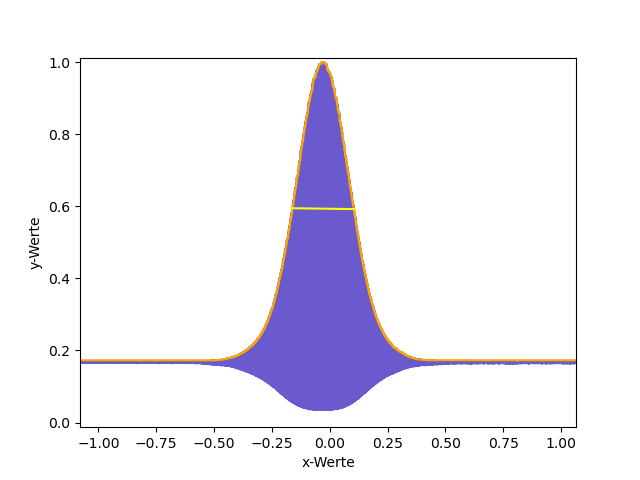
\includegraphics[width=0.7\linewidth]{images/Pulsbreite}
    \caption{
        Die Pulsbreite eines verarbeiteten Datensatzes (die Länge der Gelben Linie).
    }
    \label{fig:pulsbreite}
\end{figure}

\section{Eingabeformat}\label{sec:eingabe-format}
Wie bereits beschrieben liegen die Datensätze in Textdateien.
In diesen Dateien sind die einzelnen Messpunkte, bestehend aus \~x- und y-Wert, zeilenweise zu finden.
An erster Stelle steht der y-Wert.
Getrennt durch einen Tabulator folgt der \~x-Wert.
Zeilen die mit einem \#-Zeichen beginnen sind Kommentare und können ignoriert werden.
\begin{figure}[htb]
    \centering
    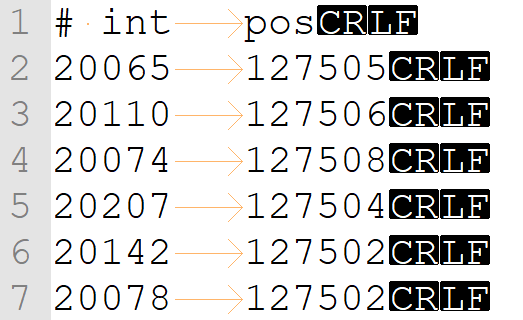
\includegraphics[width=0.5\linewidth]{images/eingabeDat_bsp}
    \caption{
        Beispielausschnitt einer Eingabedatei.
    }
    \label{fig:eingabe_dat_beispiel}
\end{figure}


\section{Ausgabeformat}\label{sec:ausgabeformat}
Nach erfolgreicher Verarbeitung werden die Ergebnisse wieder in eine Textdatei geschrieben.
Diese dateien haben den Namen der zugehörigen Eingabedatei mit dem zusätzlichen Präfix \enquote{out}.
Die Eingabedatei \enquote{1.txt} hat dann z.B. \enquote{out1.txt}.

In die erste Zeile werden die Informationen zur berechneten Pulsbreite geschrieben.
Dabei soll das folgende Format verwendet werden:
\begin{center}
    \# FWHM = <Pulsbreite:float>, <Links-Index:int>, <Rechts-Index:int>
\end{center}
In den folgenden Zeilen sollen wieder zeilenweise die verarbeiteten Messpunkte stehen.
Pro Zeile werden, jeweils getrennt durch einen Tabulator, erwartet:
\begin{itemize}[noitemsep]
    \item Der umgeformte und geglättete \~x-Wert.
    \item Der skalierte y-Wert.
    \item Der Wert der oberen Einhüllenden an der passenden Stelle.
\end{itemize}

\begin{figure}[htb]
    \centering
    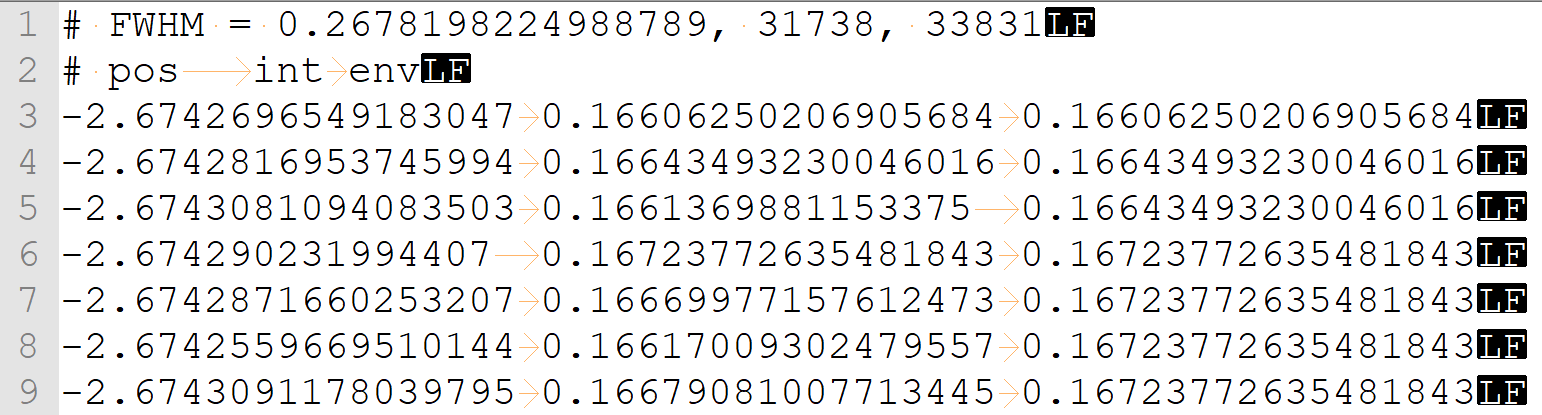
\includegraphics[width=\linewidth]{images/ausgabeDat_bsp}
    \caption{
        Beispielausschnitt einer Ausgabedatei.
    }
    \label{fig:ausgabe_dat_beispiel}
\end{figure}

\section{Fehlerarten}\label{sec:fehlerarten}
Beim ausführen des Programms kann es zu unterschiedlichen Fehlern kommen.
Diese werden im Folgenden beschrieben.

\subsection{Technische Fehler}\label{subsec:technische-fehler}
Das Programm geht davon aus, dass die Anzahl der Testdateien mit dem angegebenen Wert übereinstimmt und dass die Dateien die oben genannte Namenskonvention einhalten.
Ist das nicht der Fall, werden Zugriff auf die Dateien Fehler geworfen.
Es kann auch sein, dass eine datei beim Zugriff blockiert ist (z.B. durch ein anderes Programm oder wegen fehlenden Berechtigungen).
Dies würde ebenso zu einer Fehlersituation führen.

Auch bei der Ausgabe kann es beim Schreiben der Dateien zu technischen Fehler kommen.

\subsection{Syntaktische Fehler}\label{subsec:syntaktische-fehler}
Syntaktische Fehler treten auf, wenn die Eingabedateien nicht im richtigen Format vorliegen (Siehe Abschnitt~\ref{sec:eingabe-format}).
Z.B. wenn statt dem Tabulator ein anderes Trennzeichen verwendet wird oder mehr als zwei Einträge in einer Zeile zu finden sind.

\subsection{Semantische Fehler}\label{subsec:semantische-fehler}
Auch semantische Fehler müssen bei der Eingabe überprüft werden.
Es sind in den Eingabedateien nur positive Ganzzahlen als \~x- und y-Werte erlaubt.
Außerdem sollten mindestens 500 gültige Einträge pro Datei vorhanden sein.
Sonst kommt es beim Glätten der \~x-Werte nach der Berechnung $n = \lfloor 0.002 \cdot N \rfloor - 1$ zu Problemen.
Ist $N$ hier kleiner als 500, dann wird $n$ negative und eignet sich nicht als Obergrenze für die Summe.

\section{Fehlerbehandlung}\label{sec:fehlerbehandlung}
Die oben spezifizierten Fehler benötigen alle eine sinnvolle Fehlerbehandlung.
Diese wird nun festgelegt.

\subsection{Technische Fehler}\label{subsec:technische-fehler-behandlung}
Wenn eine Datei sich nicht zum Lesen oder Schreiben öffnen lässt, sollte eine entsprechende Meldung auf der Konsole ausgegeben werden.
Zudem sollte diese Datei in der Programmsteuerung als bearbeitet markiert werden, bzw. der Zähler der bearbeiteten Dateien hochgezähl werden.
Ansonsten würde das Programm endlos weiterlaufen.

\subsection{Syntaktische und Semantische Fehler}\label{subsec:syntaktische-semant-fehler-behandlung}
Fehlerhafte Zeilen in den Eingabedateien werden ebenfalls auf der Konsole gemeldet und für die Verarbeitung ignoriert.
Hat eine Datei in mehr als 50\% der Zeilen syntaktische oder semantische Fehler, wird sie nicht weiterverarbeitet.
Selbiges gilt, wenn weniger als 500 fehlerfreie Einträge vorhanden sind.



%\subsection{Sonderfälle}\label{subsec:sonderfaelle}
